\documentclass[12pt]{article}

\usepackage[german]{babel}
\usepackage{amsmath}
\usepackage{amssymb} % to display symbols for real numbers, integers etc. Usage: \mathbb{R}
\usepackage{graphicx}
\usepackage{listings} % to display programming code
%\usepackage[ngerman]{babel}
\usepackage{color}
\usepackage{relsize} % to display scaled math symbols (big summation symbol etc.)
\usepackage{textcomp}

\DeclareGraphicsExtensions{.pdf,.jpeg,.png}
\definecolor{listinggray}{gray}{0.9}
\definecolor{lbcolor}{rgb}{0.9,0.9,0.9}
\lstset{ % to display programming code in nice colors
	backgroundcolor=\color{lbcolor},
	tabsize=4,
	rulecolor=,
	language=matlab,
		basicstyle=\scriptsize, %for extra small font size
        upquote=true,
        aboveskip={1.5\baselineskip},
        columns=fixed,
        showstringspaces=false,
        extendedchars=true,
        breaklines=true,
        prebreak = \raisebox{0ex}[0ex][0ex]{\ensuremath{\hookleftarrow}},
		frame=single, %draw frame
        showtabs=false,
        showspaces=false,
        showstringspaces=false,
        identifierstyle=\ttfamily,
        keywordstyle=\color[rgb]{0,0,1},
        commentstyle=\color[rgb]{0.133,0.545,0.133},
        stringstyle=\color[rgb]{0.627,0.126,0.941},
        numbers=left,
        stepnumber=1,
        firstnumber=1,
        numberfirstline=true,
        linewidth=14cm,
}

\title{Uebungsblatt 3\\ \glqq Mustererkennung\grqq}
\author{J. Cavojska, N. Lehmann, R. Toudic}
\date{05.05.2015}
\begin{document}
\maketitle
%\renewcommand{\contentsname}{Table of Contents}

\tableofcontents
\newpage

\section{Aufbereitung der Daten}
\begin{lstlisting}[language=Python]
% Trainingsdaten, Testdaten und Clusterdaten laden
A = load('pendigits-training.txt');
B = load('pendigits-testing.txt');
C = load('clusters.txt');

%Dimensionen der Trainingsdaten
A_n   = size(A,2);
A_m   = size(A,1);

% Dimensionen der Testdaten
B_n   = size(B,2);
B_m   = size(B,1);

% Daten ohne die Zugliniennummer (Trainings- und Testdaten)
A_nl = A(:,1:A_n -1);
B_nl = B(:,1:B_n -1);

% Trainingsdaten aufgeteilt nach Zugliniennummer
A_0 = A((A(:,17)==0),:);
A_1 = A((A(:,17)==1),:);
A_2 = A((A(:,17)==2),:);
A_3 = A((A(:,17)==3),:); 
A_4 = A((A(:,17)==4),:);
A_5 = A((A(:,17)==5),:);
A_6 = A((A(:,17)==6),:);
A_7 = A((A(:,17)==7),:);
A_8 = A((A(:,17)==8),:);
A_9 = A((A(:,17)==9),:);

% Trainingsdaten aufgeteilt nach Zugliniennummer ohne Zugliniennummer
A_0_nl = A_0(:,1:A_n -1);
A_1_nl = A_1(:,1:A_n -1);
A_2_nl = A_2(:,1:A_n -1);
A_3_nl = A_3(:,1:A_n -1);
A_4_nl = A_4(:,1:A_n -1);
A_5_nl = A_5(:,1:A_n -1);
A_6_nl = A_6(:,1:A_n -1);
A_7_nl = A_7(:,1:A_n -1);
A_8_nl = A_8(:,1:A_n -1);
A_9_nl = A_9(:,1:A_n -1);
\end{lstlisting}
\newpage

\section{Aufgabe 1 (Multivariate Normalverteilung)}
\textit{Laden Sie die Dateien pendigits-­testing.txt​ und pendigits­training.txt​. Jede Zeile dieser Dateien ist ein Datensatz fuer einen Linienzug einer Ziffer bestehend aus 17 Zahlen, die durch Leerzeichen getrennt sind. Die ersten 16 Zahlen sind 8 X/Y ­Koordinatenpaare. Die letzte Zahl ist die Ziffer, die der Linienzug darstellen soll.\\
\\
Berechnen Sie die multivariate (mehrdimensionale) Normalverteilung​ (Erwartungswert und Kovarianzmatrix) über dem 16­-dimensionalen Koordinatenvektor jeweils fuer alle 10 Ziffern anhand der Werte aus ​pendigits­training.txt​.}
\begin{lstlisting}[language=Python]
% Erwartungswert fuer jede Koordinate fuer jeden Zug (0 bis 9)
E_A_0 = mean(A_0_nl);
E_A_1 = mean(A_1_nl);
E_A_2 = mean(A_2_nl);
E_A_3 = mean(A_3_nl);
E_A_4 = mean(A_4_nl);
E_A_5 = mean(A_5_nl);
E_A_6 = mean(A_6_nl);
E_A_7 = mean(A_7_nl);
E_A_8 = mean(A_8_nl);
E_A_9 = mean(A_9_nl);

% Kovarianzmatrix fuer jeden Zug (0 bis 9)
CVM_A_0 = cov(A_0_nl);
CVM_A_1 = cov(A_1_nl);
CVM_A_2 = cov(A_2_nl);
CVM_A_3 = cov(A_3_nl);
CVM_A_4 = cov(A_4_nl);
CVM_A_5 = cov(A_5_nl);
CVM_A_6 = cov(A_6_nl);
CVM_A_7 = cov(A_7_nl);
CVM_A_8 = cov(A_8_nl);
CVM_A_9 = cov(A_9_nl);

% Multivariante PDF generieren fuer jeden Zug (0 bis 9)
A_0_mvpdf = mvnpdf(A_0_nl, E_A_0, CVM_A_0);
A_1_mvpdf = mvnpdf(A_1_nl, E_A_1, CVM_A_1);
A_2_mvpdf = mvnpdf(A_2_nl, E_A_2, CVM_A_2);
A_3_mvpdf = mvnpdf(A_3_nl, E_A_3, CVM_A_3);
A_4_mvpdf = mvnpdf(A_4_nl, E_A_4, CVM_A_4);
A_5_mvpdf = mvnpdf(A_5_nl, E_A_5, CVM_A_5);
A_6_mvpdf = mvnpdf(A_6_nl, E_A_6, CVM_A_6);
A_7_mvpdf = mvnpdf(A_7_nl, E_A_7, CVM_A_7);
A_8_mvpdf = mvnpdf(A_8_nl, E_A_8, CVM_A_8);
A_9_mvpdf = mvnpdf(A_9_nl, E_A_9, CVM_A_9);

% A-Priori-Wahrscheinlichkeit fuer jeden Zug (0 bis 9)
A_x_apriori = 1 / length(unique(A(:,A_n)));

% A-Posteriori-Wahrscheinlichkeit fuer jeden Zug (0 bis 9)
A_0_aposteriori = A_0_mvpdf * A_x_apriori;
A_1_aposteriori = A_1_mvpdf * A_x_apriori;
A_2_aposteriori = A_2_mvpdf * A_x_apriori;
A_3_aposteriori = A_3_mvpdf * A_x_apriori;
A_4_aposteriori = A_4_mvpdf * A_x_apriori;
A_5_aposteriori = A_5_mvpdf * A_x_apriori;
A_6_aposteriori = A_6_mvpdf * A_x_apriori;
A_7_aposteriori = A_7_mvpdf * A_x_apriori;
A_8_aposteriori = A_8_mvpdf * A_x_apriori;
A_9_aposteriori = A_9_mvpdf * A_x_apriori;
\end{lstlisting}
\textit{Klassifizieren Sie die Ziffern in pendigits­testing.txt​ anhand der entsprechenden A­-posteriori­ Wahrscheinlichkeitsdichtefunktionen. Nehmen Sie dabei eine gleichverteilte A­priori ­Wahrscheinlichkeit fuer jede Ziffer an.}
\begin{lstlisting}[language=Python]
% Klassifizierung der Testdaten (Metrik: L2-Norm)
M_classify = [];
for index = 1:size(B,1)
    testData = B(index,1:B_n -1);
    
    % multivariate PDF für Testdatensatz (fuer jede Zuglinie)
    A_0_aposteriori_predict = mvnpdf(testData, E_A_0, CVM_A_0);
    A_1_aposteriori_predict = mvnpdf(testData, E_A_1, CVM_A_1);
    A_2_aposteriori_predict = mvnpdf(testData, E_A_2, CVM_A_2);
    A_3_aposteriori_predict = mvnpdf(testData, E_A_3, CVM_A_3);
    A_4_aposteriori_predict = mvnpdf(testData, E_A_4, CVM_A_4);
    A_5_aposteriori_predict = mvnpdf(testData, E_A_5, CVM_A_5);
    A_6_aposteriori_predict = mvnpdf(testData, E_A_6, CVM_A_6);
    A_7_aposteriori_predict = mvnpdf(testData, E_A_7, CVM_A_7);
    A_8_aposteriori_predict = mvnpdf(testData, E_A_8, CVM_A_8);
    A_9_aposteriori_predict = mvnpdf(testData, E_A_9, CVM_A_9);
    
    % L2 Norm der aposteriori Vorhersage
    A0_l2 = norm(A_0_aposteriori_predict);
    A1_l2 = norm(A_1_aposteriori_predict);
    A2_l2 = norm(A_2_aposteriori_predict);
    A3_l2 = norm(A_3_aposteriori_predict);
    A4_l2 = norm(A_4_aposteriori_predict);
    A5_l2 = norm(A_5_aposteriori_predict);
    A6_l2 = norm(A_6_aposteriori_predict);
    A7_l2 = norm(A_7_aposteriori_predict);
    A8_l2 = norm(A_8_aposteriori_predict);
    A9_l2 = norm(A_9_aposteriori_predict);
    
    % Bestimmung des Maximums (aposteriori Vorhersage)
    [maxValue, indexAtMaxValue] = max([A0_l2, A1_l2, A2_l2, A3_l2, A4_l2, A5_l2, A6_l2, A7_l2, A8_l2, A9_l2]);
    
    % Bayes Klassifikation (Welche aposteriori Vorhersage war die Groesste?)
    if (maxValue == A0_l2)                              % train 0 predicted
        tmpVector = [B(index,1:B_n -1),B(index,B_n),0];
        M_classify = vertcat(M_classify,tmpVector);
        
    elseif (maxValue == A1_l2)                          % train 1 predicted
        tmpVector = [B(index,1:B_n -1),B(index,B_n),1];
        M_classify = vertcat(M_classify,tmpVector);

    elseif (maxValue == A2_l2)                          % train 2 predicted
        tmpVector = [B(index,1:B_n -1),B(index,B_n),2];
        M_classify = vertcat(M_classify,tmpVector);

    elseif (maxValue == A3_l2)                          % train 3 predicted
        tmpVector = [B(index,1:B_n -1),B(index,B_n),3];
        M_classify = vertcat(M_classify,tmpVector);

    elseif (maxValue == A4_l2)                          % train 4 predicted
        tmpVector = [B(index,1:B_n -1),B(index,B_n),4];
        M_classify = vertcat(M_classify,tmpVector);

    elseif (maxValue == A5_l2)                          % train 5 predicted
        tmpVector = [B(index,1:B_n -1),B(index,B_n),5];
        M_classify = vertcat(M_classify,tmpVector);

    elseif (maxValue == A6_l2)                          % train 6 predicted
        tmpVector = [B(index,1:B_n -1),B(index,B_n),6];
        M_classify = vertcat(M_classify,tmpVector);

    elseif (maxValue == A7_l2)                          % train 7 predicted
        tmpVector = [B(index,1:B_n -1),B(index,B_n),7];
        M_classify = vertcat(M_classify,tmpVector);
    
    elseif (maxValue == A8_l2)                          % train 8 predicted
        tmpVector = [B(index,1:B_n -1),B(index,B_n),8];
        M_classify = vertcat(M_classify,tmpVector);
    
    else                                                % train 9 predicted
        tmpVector = [B(index,1:B_n -1),B(index,B_n),9];
        M_classify = vertcat(M_classify,tmpVector);

    end % end-if

end % end-for_each
\end{lstlisting}
\newpage
\textit{Geben ​Sie die Konfusionsmatrix und Klassifikationsgüte aus​.}
\begin{lstlisting}[language=Python]
% Konfusionsmatrix (Rows: actual classes, Columns: predicted classes)
%  341     0     0     0     0     0     0     0    22     0
%    0   350    12     0     1     0     0     0     1     0
%    0     8   355     0     0     0     0     1     0     0
%    0     9     0   320     0     1     0     1     0     5
%    0     0     0     0   362     0     0     0     0     2
%    0     0     0     1     0   323     0     0     2     9
%    0     0     0     0     0     0   325     0    11     0
%    0    28     0     0     0     0     0   314     5    17
%    0     0     0     0     0     0     0     0   336     0
%    0     5     0     0     0     0     0     1     1   329
knownClass = M_classify(:, B_n);
predictedClass = M_classify(:, B_n +1);
confusion_matrix = confusionmat(knownClass, predictedClass)

% Klassifikationsguete = 0.9591
M_m = size(M_classify, 1);
corret_predicted = 0;
for index = 1:M_m
    if M_classify(index, B_n) == M_classify(index, B_n +1)
        corret_predicted = corret_predicted + 1;
    end
end
classification_quality = corret_predicted / M_m
\end{lstlisting}
\newpage

\section{Aufgabe 2 (Multivariate Normalverteilung mit PCA)}
\textit{a) Geben sie die erste Hauptkomponente der Daten in pendigits­training.txt​ an.}
\begin{lstlisting}[language=Python]
% Kovarianzmatrix
CVM_A = cov(A_nl); % zentriert durch cov()
CVM_B = cov(B_nl); % zentriert durch cov()

% Eigenvektoren (VB) und Eigenwerte (DB) der Kovarianzmatrix (balanciert)
[VB,DB] = eig(CVM_A);
EigVec_CVM_A = VB; % Eigenvektoren von CVM_A
EigVal_CVM_A = DB; % Diagonalmatrix der Eigenwerte zu CVM_A

[VB,DB] = eig(CVM_B);
EigVec_CVM_B = VB; % Eigenvektoren von CVM_B
EigVal_CVM_B = DB; % Diagonalmatrix der Eigenwerte zu CVM_B

X = EigVec_CVM_A(:,[16,15,14,13,12,11,10,9,8,7,6,5,4,3,2,1]);

% get the principal component (the eigenvector with the highest eigenvalue):
% the eigenvalues in EigVal_CVM_A are already sorted (ascending), so we can just get the last column:
first_principal_component = EigVec_CVM_A(:,end)

% erste Hauptkomponente:
%  0.0713
%  0.0722
%  -0.2017
%  -0.1531
%  -0.2704
%  -0.3593
%  -0.1578
%  -0.4137
%  -0.1183
%  -0.1779
%  -0.0376
%  0.2106
%  0.0705
%  0.4627
%  0.0877
%  0.4574
\end{lstlisting}
\newpage
\textit{b) Reduzieren Sie die Dimension des pendigits-­Datensatzes mittels einer Hauptkomponentennanalyse (PCA) und klassifizieren Sie die Testdaten anhand der Trainingsdaten mit einem Bayes­-Klassifikator (wie Aufgabe 1).}
\begin{lstlisting}[language=Python]
for dim = [1:16]

    % Unterraum erzeugen
    pca_ur  = X(:,1:dim);
    
    % Abbildung der Trainingsdaten auf Unterraum
    A_0_ur = A_0_nl * pca_ur; % Datenpunkte fuer Zuglinie 0
    A_1_ur = A_1_nl * pca_ur; % Datenpunkte fuer Zuglinie 1
    A_2_ur = A_2_nl * pca_ur; % Datenpunkte fuer Zuglinie 2
    A_3_ur = A_3_nl * pca_ur; % Datenpunkte fuer Zuglinie 3
    A_4_ur = A_4_nl * pca_ur; % Datenpunkte fuer Zuglinie 4
    A_5_ur = A_5_nl * pca_ur; % Datenpunkte fuer Zuglinie 5
    A_6_ur = A_6_nl * pca_ur; % Datenpunkte fuer Zuglinie 6
    A_7_ur = A_7_nl * pca_ur; % Datenpunkte fuer Zuglinie 7
    A_8_ur = A_8_nl * pca_ur; % Datenpunkte fuer Zuglinie 8
    A_9_ur = A_9_nl * pca_ur; % Datenpunkte fuer Zuglinie 9
    
    % Abbildung der Testdaten auf Unterraum
    B_ur  = B_nl * pca_ur;
    
    % Erwartungswerte bestimmen
    E_A_0_ur = mean(A_0_ur);
    E_A_1_ur = mean(A_1_ur);
    E_A_2_ur = mean(A_2_ur);
    E_A_3_ur = mean(A_3_ur);
    E_A_4_ur = mean(A_4_ur);
    E_A_5_ur = mean(A_5_ur);
    E_A_6_ur = mean(A_6_ur);
    E_A_7_ur = mean(A_7_ur);
    E_A_8_ur = mean(A_8_ur);
    E_A_9_ur = mean(A_9_ur);
    
    % Kovarianzmatrizen bestimmen
    CVM_A_0_ur = cov(A_0_ur);
    CVM_A_1_ur = cov(A_1_ur);
    CVM_A_2_ur = cov(A_2_ur);
    CVM_A_3_ur = cov(A_3_ur);
    CVM_A_4_ur = cov(A_4_ur);
    CVM_A_5_ur = cov(A_5_ur);
    CVM_A_6_ur = cov(A_6_ur);
    CVM_A_7_ur = cov(A_7_ur);
    CVM_A_8_ur = cov(A_8_ur);
    CVM_A_9_ur = cov(A_9_ur);
    
    % Klassifizierung der Testdaten (Metrik: L2-Norm)
    M_classify = [];
    for index = 1:size(B_ur,1)
        testData = B_ur(index,:);
    
        % multivariate PDF fuer Testdatensatz (für jede Zuglinie)
        A_0_aposteriori_predict = mvnpdf(testData, E_A_0_ur, CVM_A_0_ur) * A_x_apriori;
        A_1_aposteriori_predict = mvnpdf(testData, E_A_1_ur, CVM_A_1_ur) * A_x_apriori;
        A_2_aposteriori_predict = mvnpdf(testData, E_A_2_ur, CVM_A_2_ur) * A_x_apriori;
        A_3_aposteriori_predict = mvnpdf(testData, E_A_3_ur, CVM_A_3_ur) * A_x_apriori;
        A_4_aposteriori_predict = mvnpdf(testData, E_A_4_ur, CVM_A_4_ur) * A_x_apriori;
        A_5_aposteriori_predict = mvnpdf(testData, E_A_5_ur, CVM_A_5_ur) * A_x_apriori;
        A_6_aposteriori_predict = mvnpdf(testData, E_A_6_ur, CVM_A_6_ur) * A_x_apriori;
        A_7_aposteriori_predict = mvnpdf(testData, E_A_7_ur, CVM_A_7_ur) * A_x_apriori;
        A_8_aposteriori_predict = mvnpdf(testData, E_A_8_ur, CVM_A_8_ur) * A_x_apriori;
        A_9_aposteriori_predict = mvnpdf(testData, E_A_9_ur, CVM_A_9_ur) * A_x_apriori;
    
        % L2 Norm der aposteriori Vorhersage
        A0_l2 = norm(A_0_aposteriori_predict);
        A1_l2 = norm(A_1_aposteriori_predict);
        A2_l2 = norm(A_2_aposteriori_predict);
        A3_l2 = norm(A_3_aposteriori_predict);
        A4_l2 = norm(A_4_aposteriori_predict);
        A5_l2 = norm(A_5_aposteriori_predict);
        A6_l2 = norm(A_6_aposteriori_predict);
        A7_l2 = norm(A_7_aposteriori_predict);
        A8_l2 = norm(A_8_aposteriori_predict);
        A9_l2 = norm(A_9_aposteriori_predict);
    
        % Bestimmung des Maximums (aposteriori Vorhersage)
        [maxValue, indexAtMaxValue] = max([A0_l2, A1_l2, A2_l2, A3_l2, A4_l2, A5_l2, A6_l2, A7_l2, A8_l2, A9_l2]);
    
        % Bayes Klassifikation (Welche aposteriori Vorhersage war die Groesste?)
        if (maxValue == A0_l2)       % train 0 predicted
            tmpVector = [B_ur(index,:),B(index,B_n),0];
            M_classify = vertcat(M_classify,tmpVector);
        elseif (maxValue == A1_l2)   % train 1 predicted
            tmpVector = [B_ur(index,:),B(index,B_n),1];
            M_classify = vertcat(M_classify,tmpVector);
        elseif (maxValue == A2_l2)   % train 2 predicted
            tmpVector = [B_ur(index,:),B(index,B_n),2];
            M_classify = vertcat(M_classify,tmpVector);
        elseif (maxValue == A3_l2)   % train 3 predicted
            tmpVector = [B_ur(index,:),B(index,B_n),3];
            M_classify = vertcat(M_classify,tmpVector);
        elseif (maxValue == A4_l2)   % train 4 predicted
            tmpVector = [B_ur(index,:),B(index,B_n),4];
            M_classify = vertcat(M_classify,tmpVector);
        elseif (maxValue == A5_l2)   % train 5 predicted
            tmpVector = [B_ur(index,:),B(index,B_n),5];
            M_classify = vertcat(M_classify,tmpVector);
        elseif (maxValue == A6_l2)   % train 6 predicted
            tmpVector = [B_ur(index,:),B(index,B_n),6];
            M_classify = vertcat(M_classify,tmpVector);
        elseif (maxValue == A7_l2)   % train 7 predicted
            tmpVector = [B_ur(index,:),B(index,B_n),7];
            M_classify = vertcat(M_classify,tmpVector);
        elseif (maxValue == A8_l2)   % train 8 predicted
            tmpVector = [B_ur(index,:),B(index,B_n),8];
            M_classify = vertcat(M_classify,tmpVector);
        else                         % train 9 predicted
            tmpVector = [B_ur(index,:),B(index,B_n),9];
            M_classify = vertcat(M_classify,tmpVector);
        end % end-if
    end % end-for_each
    
    M_classify_n = size(M_classify,2);
    M_classify_m = size(M_classify,1);

    % Konfusionsmatrix
    knownClass	 = M_classify(:, M_classify_n -1);
    predictedClass	 = M_classify(:, M_classify_n);
    disp(['Number of dimensions: ',num2str(dim)]);
    confusionmatrix	 = confusionmat(knownClass, predictedClass)

    % Klassifikationsguete
    corret_predicted = 0;
    for index = 1:M_classify_m
        if M_classify(index, M_classify_n -1) == M_classify(index, M_classify_n)
            corret_predicted = corret_predicted + 1;
        end
    end
    classification_quality = corret_predicted / M_classify_m
    
end % for dim
\end{lstlisting}
\newpage
\textit{Geben Sie die Klassifikationsguete fuer jede der Dimensionen von 1 bis 15 aus.}\\
\begin{lstlisting}[language=Python]
Number of dimensions: 1
classification_quality = 0.4042

Number of dimensions: 2
classification_quality = 0.6515

Number of dimensions: 3
classification_quality = 0.7882

Number of dimensions: 4
classification_quality = 0.8382

Number of dimensions: 5
classification_quality = 0.8708

Number of dimensions: 6
classification_quality = 0.8957

Number of dimensions: 7
classification_quality = 0.9062

Number of dimensions: 8
classification_quality = 0.9260

Number of dimensions: 9
classification_quality = 0.9491

Number of dimensions: 10
classification_quality = 0.9480

Number of dimensions: 11
classification_quality = 0.9537

Number of dimensions: 12
classification_quality = 0.9540

Number of dimensions: 13
classification_quality = 0.9554

Number of dimensions: 14
classification_quality = 0.9565

Number of dimensions: 15
classification_quality = 0.9594

Number of dimensions: 16
classification_quality = 0.9591
\end{lstlisting}
\newpage

\section{Aufgabe 3 (k-Means)}
\textit{Laden Sie die Datei clusters.txt​. Jede Zeile dieser Datei entspricht einem X/Y ­Koordinatenpaar. Clustern Sie den Datensatz mit dem k­-Means-­Algorithmus. Visualisieren Sie die Clusterzentren und Zuordnung der Punkte der ersten 5 Iterationsschritte mit k=3 (Also insgesamt 5 Bilder)}
\begin{lstlisting}[language=Python]
C = load('clusters.txt');
k = 3;
numIterations = 5;

mean1 = C(1,:); % mean1, selected randomly
mean2 = C(2,:); % mean2, selected randomly
mean3 = C(3,:); % mean3, selected randomly
mean1_elems = []; % elements belonging to mean1
mean2_elems = []; % elements belonging to mean2
mean3_elems = []; % elements belonging to mean3
plotArray = [];

for iter=1:numIterations
    mean1_elems = [];
    mean2_elems = [];
    mean3_elems = [];
    for elem=1:size(C,1) % iterate over all elements
        dist = sqrt(abs(C(elem,1) - mean1(:,1))^2  + abs(C(elem,2) - mean1(:,2))^2);
        closest = mean1;
        dist2 = sqrt(abs(C(elem,1) - mean2(:,1))^2  + abs(C(elem,2) - mean2(:,2))^2);
        if dist > dist2
            closest = mean2;
            dist = dist2;
        end
        dist3 = sqrt(abs(C(elem,1) - mean3(:,1))^2  + abs(C(elem,2) - mean3(:,2))^2);
        if dist > dist3
            closest = mean3;
            dist = dist3;
        end
        if closest == mean1
            mean1_elems = vertcat(mean1_elems, C(elem, :));
        elseif closest == mean2
            mean2_elems = vertcat(mean2_elems, C(elem, :));
        else
            mean3_elems = vertcat(mean3_elems, C(elem, :));
        end
    end
    mean1_elems;
    mean2_elems;
    mean3_elems;
    
    % Visualisierung der Clusterzentren
    plotOfIteration = 1; % which iteration do we want to see a plot for?
    if iter == plotOfIteration
        % x = min(mean1_elems):max(mean1_elems)
        mean1_elems_x = mean1_elems(:,1); % x coordinates of all elements belonging to mean1
        mean1_elems_y = mean1_elems(:,2); % y coordinates of all elements belonging to mean1
        mean2_elems_x = mean2_elems(:,1);
        mean2_elems_y = mean2_elems(:,2);
        mean3_elems_x = mean3_elems(:,1);
        mean3_elems_y = mean3_elems(:,2);
        scatter(mean1_elems_x, mean1_elems_y, 40, [1 0 0])
        hold on
        scatter(mean1(:,1), mean1(:,2), 60, [.3 0 0], 'filled')
        hold on
        scatter(mean2_elems_x, mean2_elems_y, 40, [0 1 0])
        hold on
        scatter(mean2(:,1), mean2(:,2), 60, [0 .3 0], 'filled')
        hold on
        scatter(mean3_elems_x, mean3_elems_y, 40, [0 0 1])
        hold on
        scatter(mean3(:,1), mean3(:,2), 60, [0 0 .3], 'filled')
    end
    
    % Berechnung der neuen Clusterzentren aus den berechneten Cluster-Datenpunkten
    mean1 = [mean(mean1_elems(:,1)), mean(mean1_elems(:,2))];
    mean2 = [mean(mean2_elems(:,1)), mean(mean2_elems(:,2))];
    mean3 = [mean(mean3_elems(:,1)), mean(mean3_elems(:,2))];
end
\end{lstlisting}
\newpage
\subsection{Grafiken zu den ersten 5 k-Means-Iterationen:}

\begin{enumerate}
\item 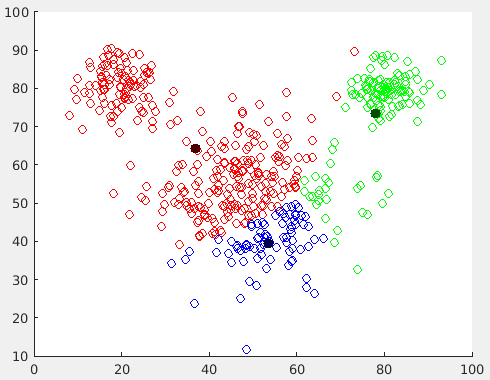
\includegraphics[width=6cm]{kmeans_iter1.png}
\item 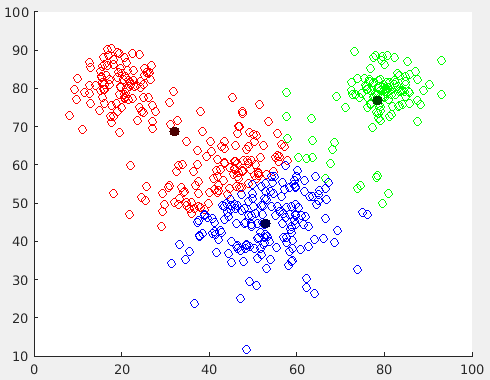
\includegraphics[width=6cm]{kmeans_iter2.png}
\item 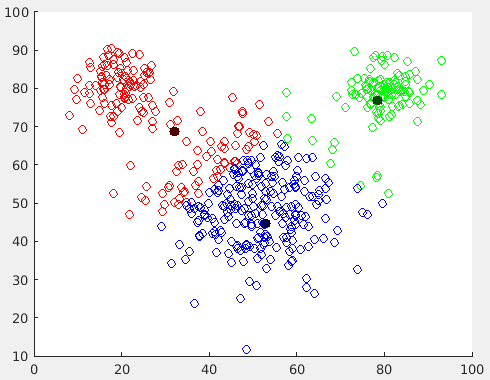
\includegraphics[width=6cm]{kmeans_iter3.png}
\item 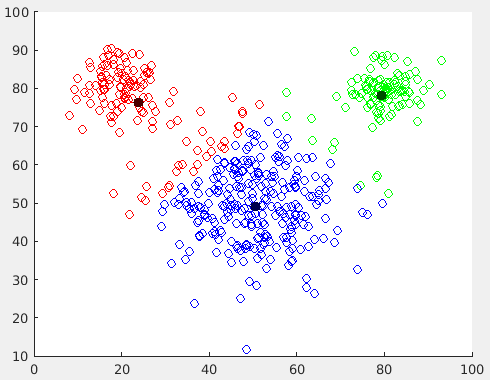
\includegraphics[width=6cm]{kmeans_iter4.png}
\item 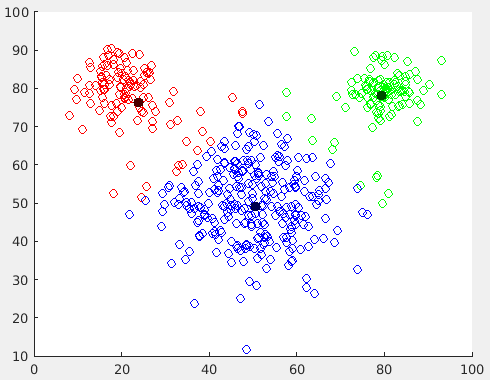
\includegraphics[width=6cm]{kmeans_iter5.png}
\end{enumerate}

\end{document}